\begin{savequote}[75mm]
If you want to keep a secret, you must also hide it from yourself.
\qauthor{George Orwell, 1984}
\end{savequote}

\chapter{Privacy in proximity based apps: the nightmare of serendipitous discovery}

\newthought{The communication possibilities} opened by on-line services are almost endless. Social media allow people every day to know more about themselves, their friends and their surroundings. To use such services, users grant them a certain level of access to their private data. This data includes details about their identity, their whereabouts and in some situations even the company they work for. This level of access is obtained leveraging on third parties, like Facebook or Google, which offer log-in technologies, allowing the application to identify the user and receive precise information about them.
Once the user grant access to their data, the application stores it and assumes control over how it is further shared. The user will never be notified again on who is accessing their data, nor if these are transferred to third parties.
We believe this can expose users of such services to privacy attacks, while in addition preventing them to retain direct control over their data and who has access to it over time.
This aspect of privacy protection is particularly relevant since usually the right to privacy is interpreted as the user's right to prevent information disclosure. On-line services use this interpretation to ask the user to access certain information, yet no concrete information is passed on how the data will be used or stored. Furthermore, these services are often designed as mobile applications where all the devices installing the app communicate with a centralised server and constantly exchange users' information, eventually allowing for unknown third parties, or potential attackers, to fetch and store this data. In addition, this information is often shared with insecure communication through the HTTP protocol, making it possible for a malicious entity to intercept these communication and steal user data.

We have observed how proximity-based social applications have access to certain identity information that could lead a possible privacy attacker to easily identify users and link their on-line profiles to physical identities. In our study we analyse a set of popular dating application, which are built on the assumption that users can preserve a certain level of privacy by only sharing their relative distance with other users on the platform. Furthermore, the user also shares Facebook likes or common categories of interests.

These application are built on the notion of serendipitous discovery of people, places and interests around the user's surrounding.  We consider these applications an example of how many privacy violation users are subjected to without being aware of it. Furthermore, this scenario offers a playground to prove how little details about the user's whereabouts and personal sensitive information are needed to track the user and discover their real identities.  For example, we prove how the user's relative distance or their first name and what common interest their share on Facebook, can allow an attacker to follow them along the day and across their movements, or even profile their full interests and discover personal details about them.

\section{Background}
\noindent
On-line communications in general and social media in particular, are increasingly opening up new possibilities for users to share and interact with people and content on-line. At the same time, social networking services collect and share valuable information regarding locations, browsing habits, communication records, health information, financial information, and general preferences regarding user on-line and offline activities. This level of access is often directly granted from the user of such services, although the privacy and sensitiveness of the information becoming accessible to third parties can be easily overlooked.

Furthermore, social networks are no longer a novelty and user have become used to share their information with both social relationships as well as third party applications. Leveraging on this perception of social media by Internet users, another class of applications is being developed based on the concept of ~\emph{serendipitous} discoveries. The idea of ~\emph{serendipity} in mobile applications wants the user to accidentally discover people, places and/or interests around them, by using passive geo-localisation and recommendation systems. Passive geo-localisation is a mechanism using the ability of mobile devices to know the user's position without having to constantly asking for it. Technologies that provide this capability are GPS, wireless and mobile networks, iBeacon and so on.

To present the user with a tailored and seamless experience, serendipity applications need to learn the user's preferences and interests. This is usually accomplished by connecting several of the user's identities on other social networks. A typical example is asking the user to register onto an application through their Facebook, Twitter, or Google+ accounts. This technique usually consists in a variant of the OAuth2.0 protocol used to confirm a person's identity and to control what data they will share with the application requesting log-in.

We have specifically analysed Facebook log-in since it was the common log-in mechanism offered in all applications examined, although the same functionality apply for other third party log-in mechanisms. Facebook log-in provides both authentication and authorisation. The mechanism is used on the web as well as on iOS and Android, although on those platforms the primary mechanism uses the native Facebook application instead of the web API.

When an application is connected to the user's Facebook profile using Facebook log-in, it can always access their \emph{public profile} information. Facebook consider this information public and will not apply any restriction on it. Information that is shared with the public profile vary from user to user and depends on their privacy settings. By default, the Facebook public profile includes some basic attributes about the person such as the user's age range, language and country, but also the name, gender, username and user ID (account number), profile picture, cover photo and networks.

An application may also ask for more information about the user. These can include the list of friends using the app, their email, the events that they are attending, their hometown or the things they have liked. This information can be obtained by requesting for optional permissions, which are asked for during log-in process. Apps can also ask for additional permissions later, after a person has logged in.

The information obtained from Facebook is often displayed on the application platform or used to match people with similar interests, thus giving away more hints about an individual real identity. For example, a user \emph{swiping} through other people on \emph{Tinder}~\cite{tinder} will know if they have liked similar pages on Facebook.
These hints or traces can be used to further identify that individual on other platforms. In fact, this information crossed with the city the user lives in, the user's photo, and their first name could already be enough to identify their Facebook profile.

The attacker could hence use what they know about the user to identify a number of profiles of people living in a certain city. A query of the form \emph{people named John who live in Barcelona and like surfing and volleyball} could be used to restrict the attacker's search space to a smaller number of profiles. Finally, since these applications tend to fetch the profile photo directly from Facebook, the actual user profile can be identified by matching the two profile pictures.

Notice that while some queries might seem very generic, some others might already restrict significantly the set of targeted profiles. It is particularly concerning in fact that these applications might be used to target specific individuals with the objective to reach confidential information about their actual job or company they work for, as reported recently by IBM in a report about security of dating apps~\cite{ibm2015report}.

The ubiquitous streams of data that users create while they use different application can be seen as a network of interconnected data snippets. Information shared on the web can be linked together so that it is possible to construct semantic connections between user's activity data. A possible attacker could therefore try to link data between different source of information to identify and target users both on-line and offline. Users become more frequently exposed to social engineering attacks that can now leverage on facts gathered on-line about their personal offline lives.

In this chapter we formalise an attack showing how proximity based social application are inherently insecure. Our attack retrieves information about nearby users, stores certain information about them, and subsequently uses these to retrieve their updated profiles at regular intervals. Our attacker agent is also able to change their relative position at will and therefore can easily perform a multilateration attack and identify the victim position with a arbitrary precision. Furthermore, the attacker can keep following the user, eventually categorising their interests, movements and even identifying their Points of Interest (POI) around the city.

Therefore, we build a Social Graph attack using Facebook likes to know the victim interests. The applications examined, in fact, allow the attacker to know ~\emph{what they have in common} with the victim and use the known expressed interests to identify the user's Facebook profile through their Graph Search while also profiling individuals nearby.

\section{Modelling the location probe method}
\label{sec:loc-probe}
\noindent
Proximity based social application collect users' positions and share their relative distances. We show how it is possible to build a multilateration attack able to identify the actual user position with arbitrary precision.

Multilateration is a navigation technique, often used in radio navigation systems, based on the measurement of the difference in distance to two or more stations, whose locations are known. The stations also produce a certain signal at a known time.\

In our scenario, the signal is replaced by the user distance from the attacker and time is given by the timestamp of the user latest activity. Please note that, multilateration is not concerned with measurements of absolute distance or angle between parties, but with measuring the difference in distance between two stations which results in an infinite number of locations that satisfy the measurement. All these possible locations form a hyperbolic curve. Multilateration therefore relies on multiple measurements to locate the exact location along that curve. In fact, a second measurement taken to a different pair of stations will produce a second curve, which intersects with the first. When the two curves are compared, a small number of possible locations are revealed.

If the attacker is able to retrieve an arbitrary number of samples of the user distance, either by changing their relative location or by sampling their distance with the victim with a number of malicious mobile client infiltrating the platform, the multilateration attack can be made arbitrary precise.

Our location probe method uses a simple multilateration algorithm. At the first step, locations expressed as longitude and latitude coordinates are translated to cartesian coordinates. We then calculate the estimated distance and minimise the linear norm between calculated distance and estimated distance by sensing the total error. We could have considered the total squared error between the estimated and actual distance, however in this contest we have concentrated on demonstrating that the attack is actually feasible, rather then on accuracy or performance of the algorithm (Fig.~\ref{fig:comp_time}).

\begin{figure}[t]
\centering
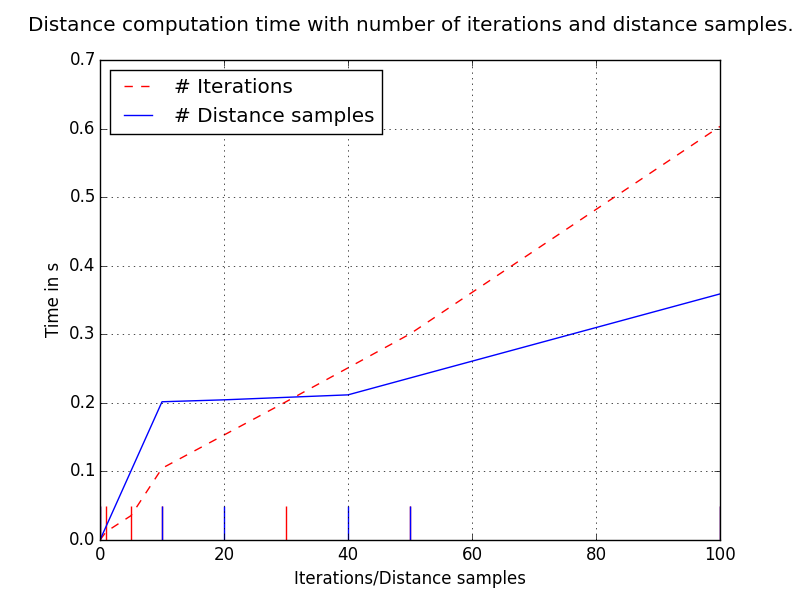
\includegraphics[width=90mm]{figures/figure_time.png}
\caption[Computational time needed to estimate a user position.]{The image illustrates the time needed to compute a user position estimation based on the number of distance samples and the number of iterations of the algorithm. It is important to note how the number of distance samples does not affect the algorithm performances. The example was executed on a Apple Computer with 3 GHz Intel Core i7 Processor.
\label{fig:comp_time}}
\end{figure}

\section{Modelling the user activity profile}
\label{sec:activity-profile}
\noindent
We model the user's activity as series of events belonging to a certain identity. Each event is a document containing different information. We can formally define this a hypermedia document i.e. an object possibly containing graphics, audio, video, plain text and hyperlinks. We call the hyperlinks selectors and we use these to build the connections between the user's different identities or events. Each identity is a profile that the user has created onto a service or platform. This can be an application account or a social network account, such as their LinkedIn or Facebook unique IDs.

Each event is the result of the user performing an action. For the purpose of this study we have consider an action as resulting using an application or a service. An action is the activity of interacting with a mobile application or \emph{liking} a resource on a social network, i.e. directly expressing an interest, or the fact that a user has updated their location at a certain time.

Formally it is possible to model the graph of the events pertaining to a user as an hypergraph, where each edge can connect any number of vertices, and the root is first event in the series.  A hypergraph $H$ is a pair $H = (X,E)$ where $X$ is a set of nodes (the events in the model), and $E$ is a set of non-­empty subsets of $X$ called hyperedges or edges. Hypergraphs are a generalisation of a graph structure and provide a reasonable representation of the connections between the different events resulting of the actions performed by the user.

We find that this model is able to express the user's on-line footprint as a collection of traces left across different services. Furthermore, by using a hypergraph model we are able to grasp the connections between the different profiles and features.

This results in the possibility to profile users based on chosen selectors. For example, we might want to trace all users who have been in the radius of 500 meters to a certain location, or all the users in a certain neighbourhood who \emph{like} a selected Facebook page.

\subsection{Adversary model}

In view of the assumptions described in the previous section, our privacy attacker boils down to an entity that aims to identify users and link their on-line profile to their physical identity. To achieve this objective, the attacker possess a Facebook profile. This profile is used in the first place to register to the application analysed in this study since all three use Facebook log-in as a personalised way for user to register and sign in.

\section{Experimental results}
\label{sec:exp-results}
\noindent
We have analysed 250 users from a set of social proximity applications (Table: ~\ref{table:violations}). All applications examined are matchmaking mobile platforms which uses geolocation technology. Users can use their location and preferences to search for interesting people in a specific radius. All applications use Facebook profiles to allow their users to log-in but also to gather basic information and analyse users' social graph. The information collected are then used to match candidates who are most likely to be compatible based on geographical location, number of mutual friends, and common interests.

\begin{table*}[ht]
\centering
\caption{Information regarding active users per application.}
\def\arraystretch{2.0}
\begin{tabular}{| c | c |}
  \hline
    Application 				& Users  \\
  \hline
  \hline
    Tinder~\cite{tinder}		& 10 Million active~\cite{tinderusers} 	\\
    Happn~\cite{happn} 		& ~ 700.000~\cite{happnusers} 				\\
    Lovoo~\cite{lovoo} 		& ~ 24 Million registered~\cite{lovoousers}		\\
    Grindr~\cite{grindr} 		& ~ 2,35 Million active~\cite{grindrusers}\\
    Badoo~\cite{badoo}	 	& 200 million registered~\cite{badoousers}	\\
  \hline
\end{tabular}
\label{table:apps}
\end{table*}

\begin{table*}[ht]
\centering
\caption{Information regarding the applications analysed}
\def\arraystretch{2.0}
\begin{tabular}{| c | c | c | c | c | c | c | c | c |}
  \hline
    Application 				& 	 Fb ID 		& 	 Loc.	 	& 	 Distance		&  	User Pref.      & 	 Full Name 	&  	Birth-date 	     & User tracking \\
  \hline
  \hline
    Tinder~\cite{tinder} 	& 	\ding{55} (1) 		& 	\ding{55} 		 &	 \ding{51} 		& \ding{51}	      & 	\ding{55} (2)	&	\ding{55} (3)  &		\ding{51}		\\
    Happn~\cite{happn} 		& 	\ding{51} (1)		& 	\ding{55} 	 	 &	 \ding{51} 		& \ding{51}	      & 	\ding{55} (2)	&	\ding{55}	     &		\ding{51}		\\
    Lovoo~\cite{lovoo} 		& 	\ding{55} (1)		& 	\ding{55}		 & 	\ding{51} 		& \ding{51}	      & 	\ding{55} (2)	&	\ding{55}	     &		\ding{51}		\\
    Grindr~\cite{grindr} 	& 	\ding{55} (1)		& 	\ding{55}	 	 & 	\ding{55} 		& \ding{51}	      & 	\ding{55}		&	\ding{55}	     &		\ding{55} 		\\
    Badoo~\cite{badoo}	 & 	\ding{55} (1)		& 	\ding{55}	 	 & 	\ding{51}(4) 	& \ding{51}	      & 	\ding{55} (2)	&	\ding{55}	     &		\ding{51} (6)	\\
  \hline
\end{tabular}
\label{table:violations}
\\[2.5pt]
 \begin{flushleft}
(1) Facebook ID is not exposed directly but it can be identified by crossing information like the user Facebook's likes, first name and year of birth. \\
(2) Only first name is shared. \\
(3) A fuzzy birthdate randomised in a range of two weeks is used. Real birthdate can be inferred by using Facebook Graph Search, depending on the victim's Facebook privacy settings. \\
(4) Offers option not to share distance. \\
(5) Asks for zodiac sign. \\
(6) Distance is shared for some users so it is theoretically possible.\\
\end{flushleft}
\end{table*}

These applications present the user with the possibility to interact with other users by starting conversation or expressing their interests in them.

\subsection{Information collection}
\noindent
Information collection is possible on these applications through different techniques. For the purpose of this study we have intercepted APIs call from mobile devices through Men In The Middle (MITM) attack in some occasions, and interacted with the APIs directly in other occasions.
\noindent
It is important to note that even when the application prevents an attacker from exploiting their APIs, a malicious entity could still use a multitude of profiles to cross gather information about users on the platforms.

\subsection{Information processing}
\noindent
We have performed two types of attack on the set of application examined, namely a multilateration attack and a social graph attack.

\subsubsection{Multilateration attack}
\noindent
Once we posses the user's id on the specific application we are able to query their APIs and update our information about the user constantly. Furthermore we are also able to change our own location on the platform to a certain extent.
\noindent
By measuring the relative distance to the victim we were able to identify their actual position with arbitrary precision. Furthermore, the same technique was used to ~\emph{follow} users across a specific amount of time by retrieving their profile information at regular interval.
\noindent
This type of attacks can be easily overlooked in densely populated cities but might become a serious privacy breach in rural areas.

\begin{figure}[t]
\centering
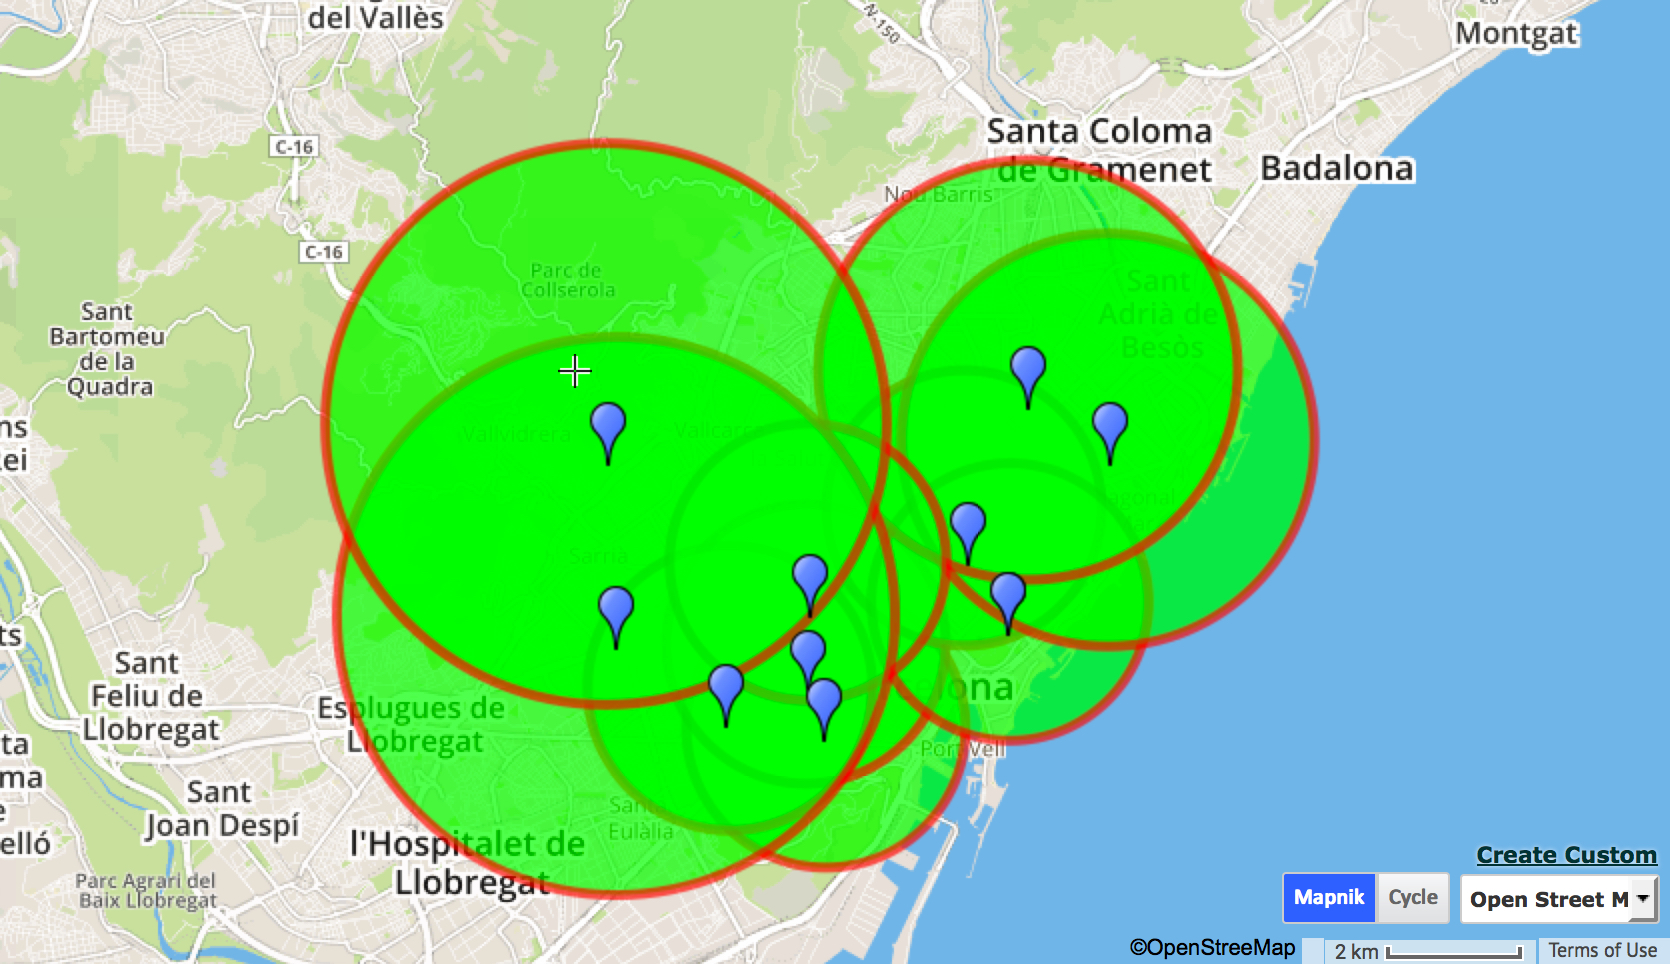
\includegraphics[width=90mm]{figures/user_mlat.jpg}
\caption[Location samples for a single user.]{The image illustrates location samples with radii used to compute actual position estimation for one user across the city of Barcelona, Spain.}
\label{fig:mlat}
\end{figure}

\subsubsection{Hyper graph attack}
\noindent
The application examined for the scope of this study use the user's Facebook token to authenticate and/or authorise the application to request and obtain certain information about the user.
An attacker could then use their own Facebook profile token to make request to the application server through their APIs, pretending to send the request from the app installed in a mobile device. This allows the attacker to receive all the information that users have shared with the platform and that are constantly exchanged with the application.

When the victim's Facebook id is shared through the application, the attacker can directly access and potentially use information publicly shared through the Facebook profile. In this situation the attacker could easily construct a complete graph of the user's preferences and social connections through the information that are public available through Facebook APIs.

When the victim's Facebook id is not directly shared, the application still disclose some information about the victim. This information include: the user first name and a set of photos, birthdate, randomised in a range of 15 days, and the Facebook pages that both the victim and the attacker have liked.

The victim preferences could then be used to identifies their Facebook profile. It is in fact estimated that Facebook posses 1.35 billion active users, of these, between 10\% and 7\% like one of the top 10 Facebook pages with most likes~\cite{pagedata}. We have collected a set of 250 Tinder users only in the city of Barcelona, of these 20\% where sharing at least one interest with the attacker profile (Fig.~\ref{fig:connections}).

Furthermore Facebook graph search allows any users to answer certain information about Facebook profiles. An example of a graph search on Facebook could be: \emph{People who like Shakira and are named "John" and like Manchester United and been born in 1979}. This will create a pool of potential candidates. The list can be reduced by using Facebook reverse graph search, i.e. search for \emph{Interests liked by people who like Shakira and are named "John" and like Manchester United and been born in 1979}.  This will instead return a list of interests that the attacker can like on Facebook. Therefore, the attacker will return to query Tinder and find out if the number of interests in common with the victim has grown and which pages they now have in common. The attacker can therefore use the new information to further identify the victim profile on Facebook and potentially their friends (Fig.~\ref{fig:fgs}).

It is important to note that some applications might request information outside of Facebook public profile. Therefore, even if the victim has tailored their privacy settings to prevent some information to be leaked, the application can be used to access data that would be otherwise be kept private.

\begin{figure}[t]
\centering
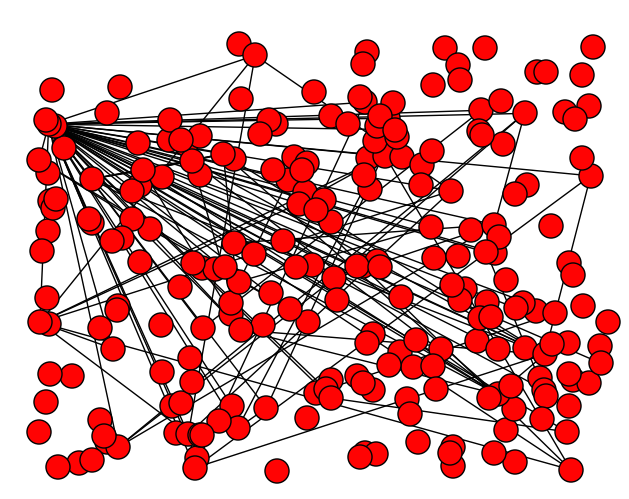
\includegraphics[width=90mm]{figures/figure_connections.png}
\caption[Facebook pages likes by Tinder users.]{The image shows how it is possible to show connections for the population of users on Tinder for a certain area. Here we have collected Facebook pages liked by users in Barcelona and connected users or group of users, if they like the same page.}\label{fig:connections}
\end{figure}

\begin{figure}[tb!]
\centering\hspace*{\fill}
{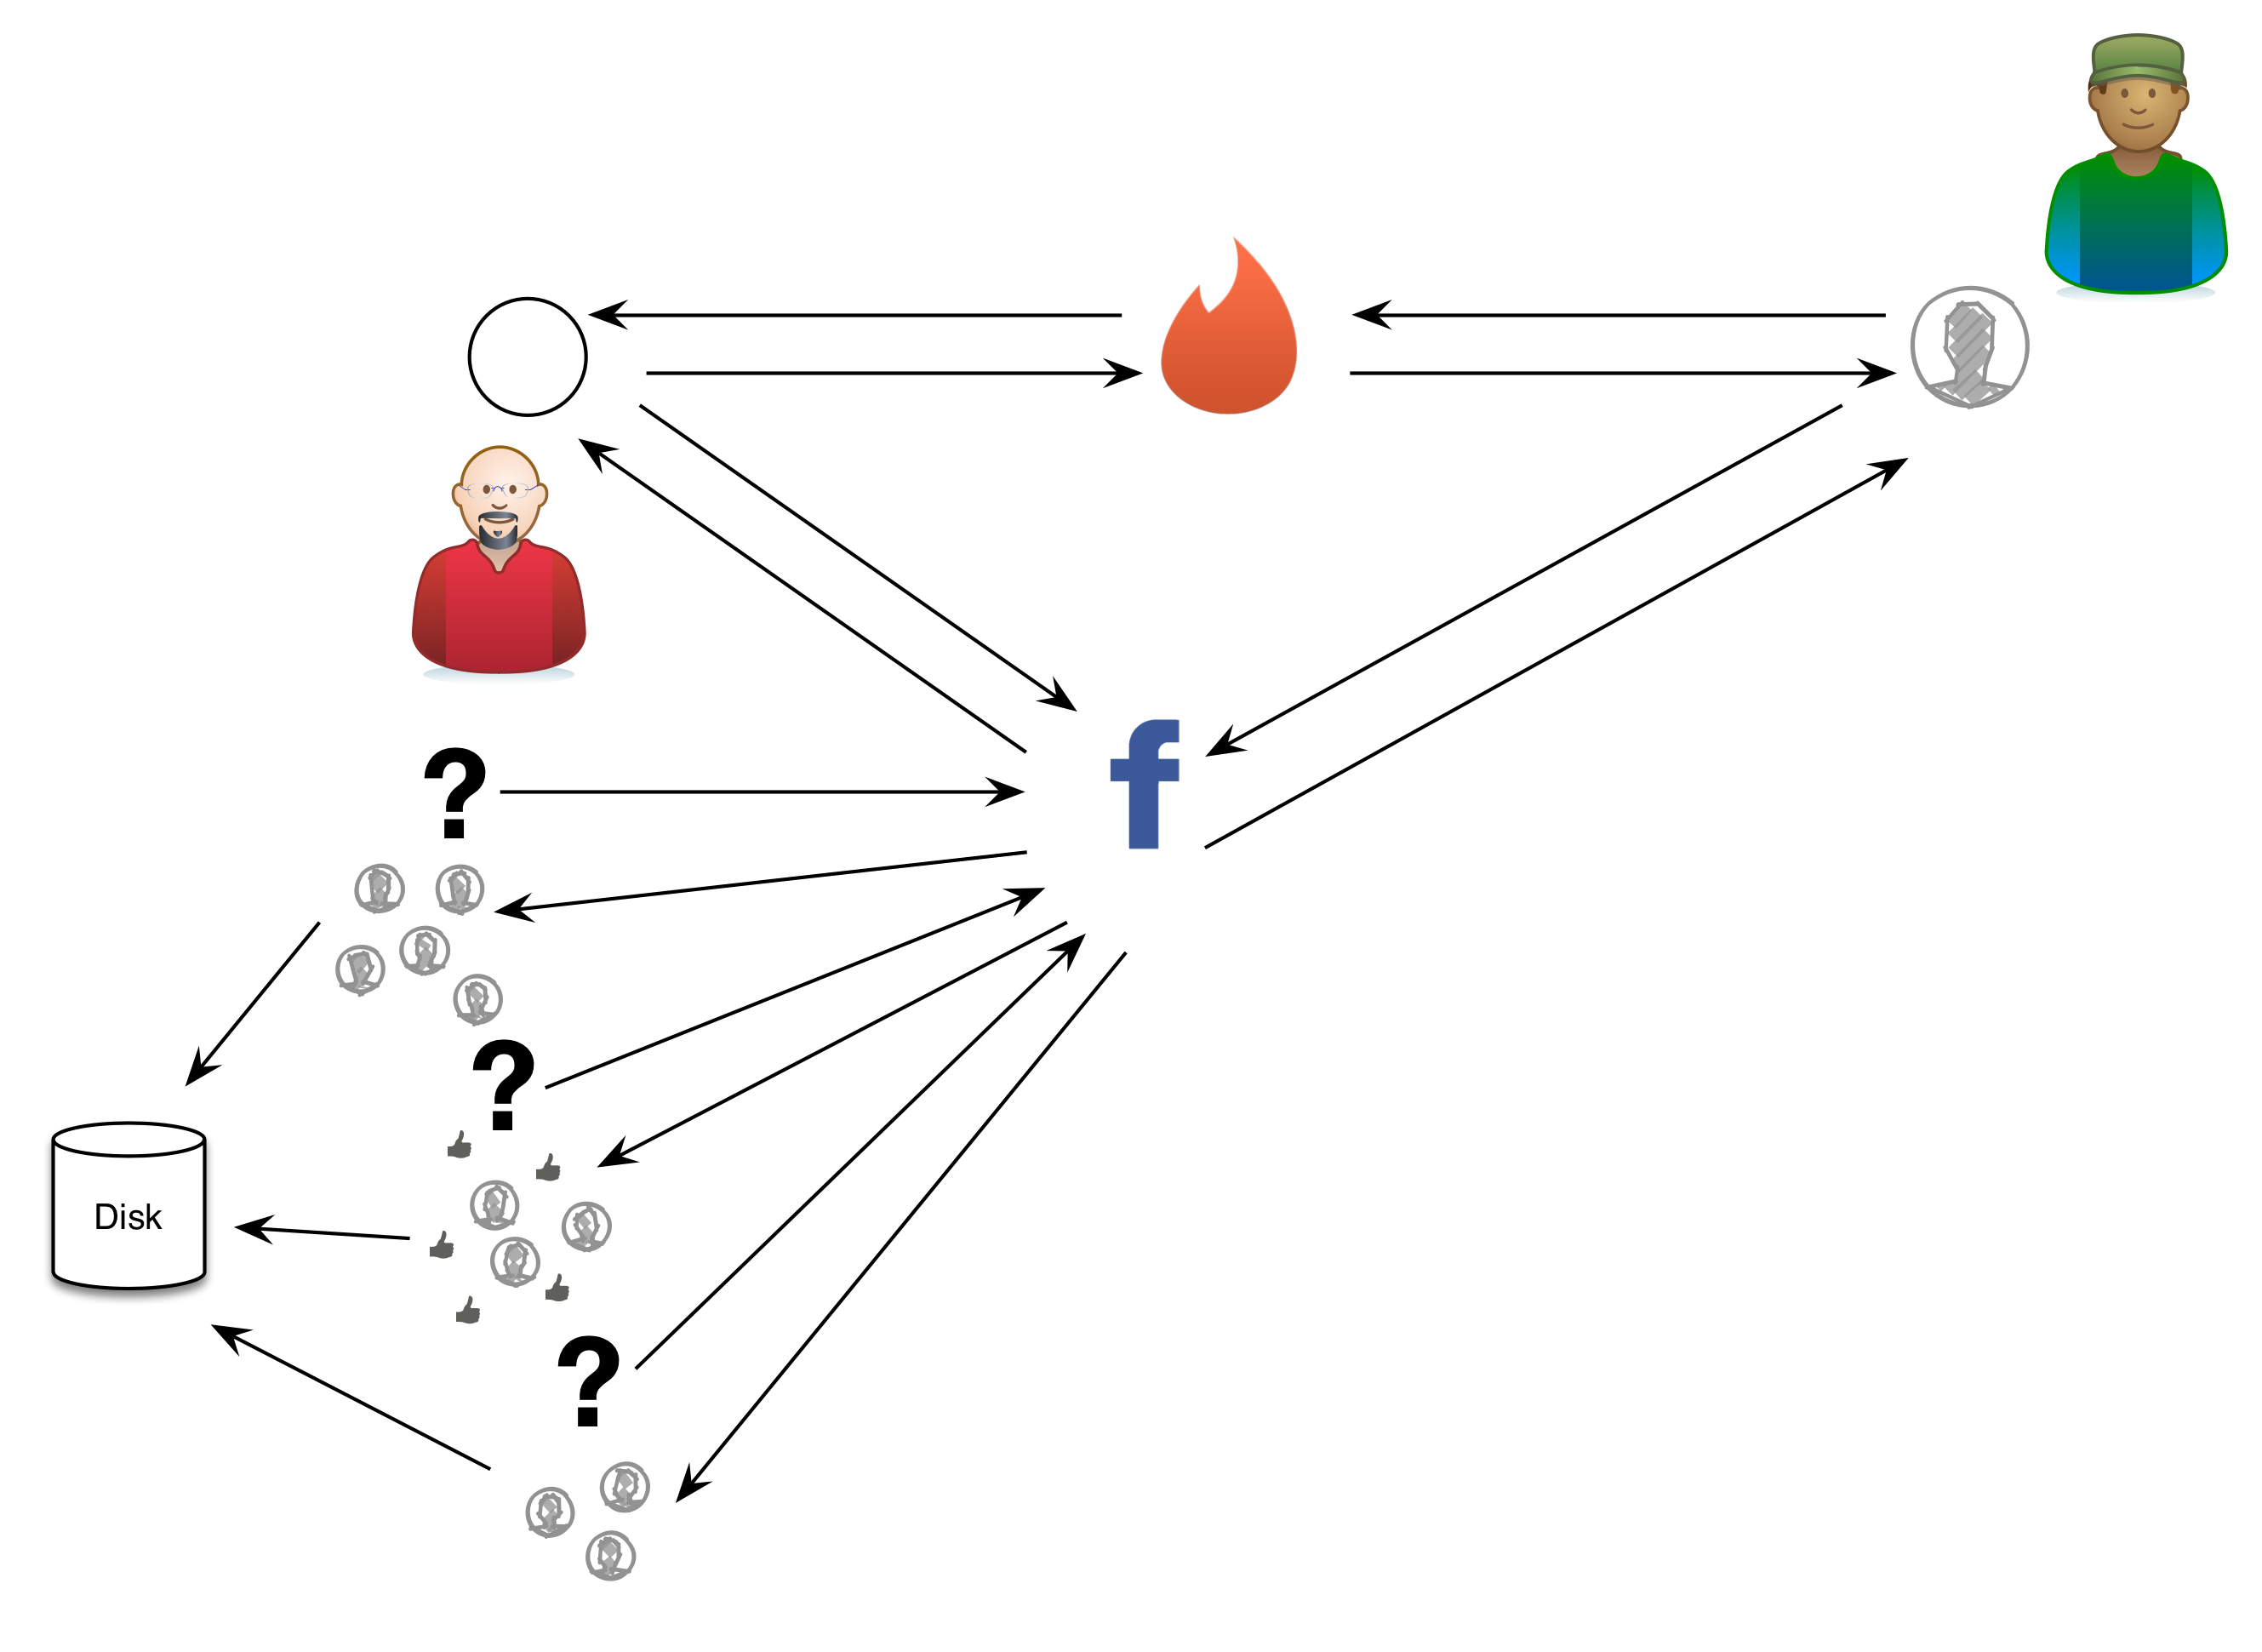
\includegraphics[width=90mm]{figures/attack_scenario.png}%
\label{graph}}\hspace*{\fill}
\caption[Social Graph attack]{The image represents a Social Graph attack where an attacker sends queries Facebook asking question about a Tinder profile. The attacker is able to restrict the pool of potential candidates and eventually identify the victim's actual Facebook id. Furthermore the attacker is able to store information about the user that can be updated at a later time by querying the third party application.}
\label{fig:fgs}
\end{figure}

\subsection{Information dissemination}
\noindent
Proximity-based social applications, in their current implementation, represent a gateway to access data about individuals. Information dissemination can therefore be accomplished both for large group of people with the purpose of targeting them, as well as for specific victims.
Identifying and disclosing the presence of a certain person on a match making application could be enough to influence the opinion of that individual among their social relationships.

\subsection{Invasion}
Once a user location has being inferred, we can continue tracking the same users and their preferences for an unlimited amount of fetches. This could easily lead to identification of the user habit and where-about at different moment of the day, possibly uncovering their home and work locations and more information about the user.

\section{Mitigation possibilities}
\noindent
Application developers could implement a number of techniques that would mitigate the actions of a possible attacker. Firstly, in their current implementation, the applications examined probe the user device for location information with the maximum precision possible. This information is then transferred to the server and the relative distance between users is returned to be displayed. Yet, for most of the application functionality this precision is not needed, and a lower precision could be used and sent to the server. This would make position attacks more difficult to perform.

Secondly, to sparkle interest between users, social proximity application often share common Facebook pages between parties involved. This information can then be used to easily identify unique Facebook accounts. Instead, the app could opt to display only the category of interest to which the Facebook page belongs. This way a possible attacker would not know what actual pages the user has liked.

Thirdly, an individual birth-date if combined with their location and first and/or last name can be used to infer sensitive information about them. Therefore even sharing the user's zodiac sign with passive observer need to be considered potentially dangerous for the final user's privacy.

To conclude, to avoid exposing users to direct threats of \emph{collection} and \emph{processing} of private information, mobile apps should have the option not to supply any personal details to the platform. Users should not obliged to disclose their personal data. To avoid \emph{dissemination} and \emph{invasion}, user data collected by mobile applications should be communicated encrypted to the server.

\section{Discussion}
\noindent
A new class of social application uses the users' actual location to provide personalised recommendation and allow for new interactions especially in urban settings. We have shown how these applications can expose their users to different privacy attacks that can be easily overlooked.

We have analysed a set of  popular dating application, and observed how proximity-based social applications have access to certain identity information that could lead a possible privacy attacker to easily identify users on Facebook and link their on-line profiles to physical identities.

Furthermore we have shown how users constantly sharing their relative distance to other users can be ~\emph{followed} by an attacker in their movement without their knowledge. We have demonstrated how this information can be used for a multilateration attack with arbitrary precision. There is in fact no restriction to the number of distance samples that a possible attacker might be able to measure.

We followed a formal framework to identify the classes of privacy violation to which users are subjected to without being aware of it and we have shown how these violations can all be carried out for the applications examined.

This shows how using third party profiles to provide access to a specific applications may cause a security \emph{honey pot} for a possible attacker.

We have also stressed how In order to make the registration process easier, these applications often leverage on third party services to provide a log-in mechanism, while at the same time acquiring certain private information about their new users. The third parties used are often services such as Facebook or Google, and the information accessed concern the public profile of the users on such platforms.

While this technique certainly allows people to quickly sign up to an application and create a new profile, it also creates different privacy threats for users of such services. Primarily, it concerns who can gain access to such data and how information shared with third parties can also be stored and eventually transferred without the user explicit consent.

We have then used Facebook graph search to build a hyper graph of the user identity starting from few information that were shared through a third application. This shows how each information can be used as a selector to further identify a different piece of the whole user identity and can be used to target the user in real life.